\section{Theory and stuff}

general architecture, oracle, it’s responsibilities, queries, piggybacking on VM
pauses, changes => effects => queries structure


\section{More stuff}
changes => effects => queries list, implementation details. 

Dynamic update of an application is aq non-deterministic process, which success
heavily depends on the state of the application at the moment of the update.
Prior
research\footnote{\url{http://www.researchgate.net/publication/220875483_Run-time_phenomena_in_dynamic_software_updating_causes_and_effects}}
has identified that certain run-time phenomena might occur during the further
run of the updated application. These phenomena could not be the intended
behavior programmed into the application itself but rather an artifact of the
dynamic update.

Consider the following manually created list of the run-time implications of the updating. 

\begin{figure}[ht!]
\begin{center}
\leavevmode
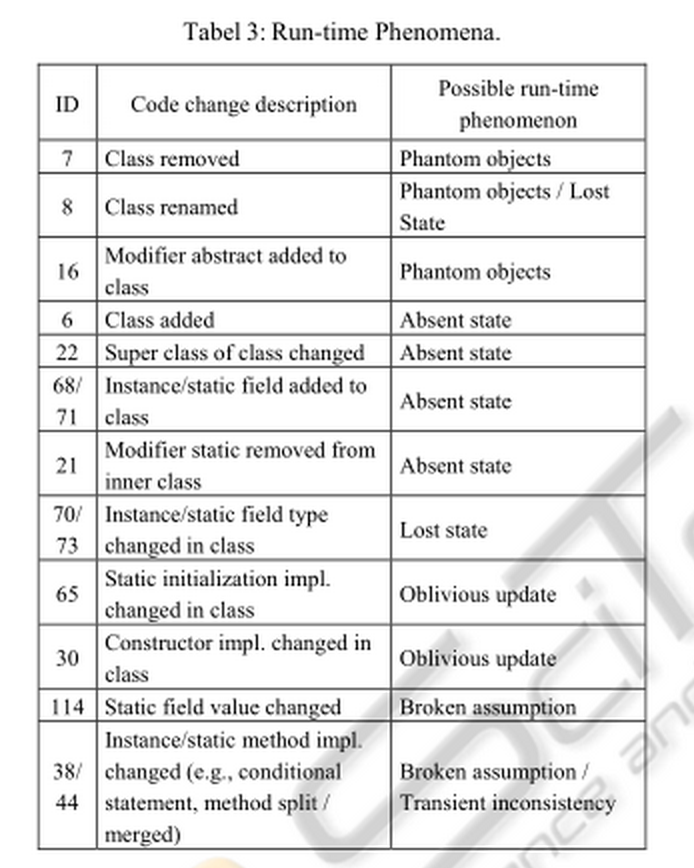
\includegraphics[scale=0.6]{../images/fig1.png}
\end{center}
\caption{Possible run-time implications of updating a Java program.
\label{possible_changes}}
\end{figure}

Note that these effects were observed during sequential update of the Breakout
application through multiple versions that contained non-trivial changes to the
application codebase.

\begin{figure}[ht!]
\begin{center}
\leavevmode
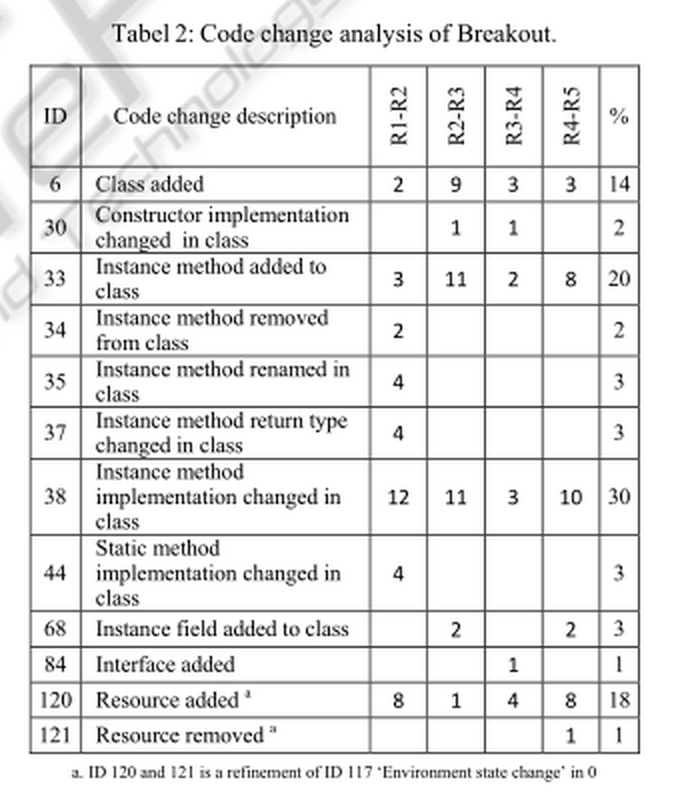
\includegraphics[scale=0.6]{../images/fig2.png}
\end{center}
\caption{Change analysis of Breakout updates.
\label{manual_change_analysis}}
\end{figure}

It is important to note that these effects are probable, but not inevitable.
Consider the “modifier abstract added to the class” change and its “phantom
objects” effect. If the class has not been instantiated or all instances of the
class were garbage collected prior to updating, the effect of having phantom
objects, which could not be instantiated in the new version of the code, will
neither be present in the updated version.
On of the challenges of the DSU is to predict and possibly minimize the
probability of the effects appearing after the update.

Below is a list of changes to the application level classes that can occur in the JVM setting.
\begin{itemize}
  \item Changes to method bodies		
  \item Adding/removing Methods		
  \item Adding/removing constructors		
  \item Adding/removing fields		
  \item Adding/removing classes		
  \item Adding/removing annotations		
  \item Changing static field value		
  \item Adding/removing enum values		
  \item Changing interfaces		
  \item Replacing superclass		
  \item Adding/removing implemented interfaces
\end{itemize}

Our approach to predicting the probability of certain effects being observed
after the update is to enumerate the effects a given change can cause and create
a list of queries to a central oracle to determine if given change will cause
given effect under the current application state.

Below we list queries that the oracle can answer:
\begin{itemize}
  \item Is class T loaded into the JVM? 
  \item Are there any loaded subclasses of class T? 
  \item Are there currently reachable objects of class T (or any subclass of T)? 
  \item Does an object of class T with a field F instantiated to a non-default
value exist?
\end{itemize}
 
The exact implementation of such oracle is described later in the paper. For now
we provide a list of effects that possible changes are responsible for and a
translation of the effects into predicates constructed from the queries listed
above.

For example:
Change: Instance field F added to the class T with default value V. 
Effect: Absent state (already instantiated objects will not have the field instantiated)
Predicate to determine the observability of the effect: 
\begin{itemize}
  \item Is class T loaded into the JVM and
  \item Are there currently reachable objects of class T (or any subclass of T)?  
\end{itemize}

If the oracle evaluates the predicate as truthful, the effect will be observed
and updating application given current state is not safe. However, it is
important to notice, that the current state of the application can change and it
might be possible to safely update the application later. For example when all
instances of class T are garbage collected and do not pose any threat.

There exist static analysis tools that given the old and new versions of the
packaged Java application can list changes that are between these versions.

When our framework receives both old and new versions of the application, it
determines the changes between these versions. Then it queries the oracle
repeatedly to assess if the current application state does lead to any effects
of the changes being observable. If there is no observable effects the update is
applied and the new version of the application continues to run.
If the update is not happening for a considerable amount of time, currently the
updating framework logs the error and stops trying to proceed with the given
update. Further development can improve this behavior to allow updates when some
of the effects are observable or when given a more complex query system even
further.